\documentclass[../main.tex]{subfiles}
\graphicspath{{\subfix{../images/}}}
\begin{document}

%%%%%%%%%%%%%%%%%%%%%%%%%%%%%%%%%%%%%%%%%%%%%%%%%%%%%%%%
% \subsection{Results: Temporal Synchronization} \label{results)time_sync_cam}

An initial evaluation of the video stream and time-stamping system was conducted under conditions that simulated expected network load conditions.
Video data was recorded for 14.5 seconds at 10 \ac{fps} (twice the anticipated operational rate) for a total of 8,720 frames. 
The NVIDIA computer in the camera enclosure was accessed via SSH terminal and displayed a log of each timestamp being recorded and sent over the RTSP video stream. 
Similarly, the Atlas PC was connected to via SSH and displayed the timestamp being received over the RTSP video stream.
This data was also logged in a text file on the respective machines and compared for analysis. 
To ensure real-world clock precision, a real-time clock was set up in front of the camera displaying the current time, and transmitted as the subject of the video feed. An image of this setup is presented in Figure~\ref{fig:time_sync1}
This allows for any internal clock drift to easily be identified by comparing the transmitted timestamp to the time displayed in the video itself.

\begin{figure}[htbp]
    \centering
    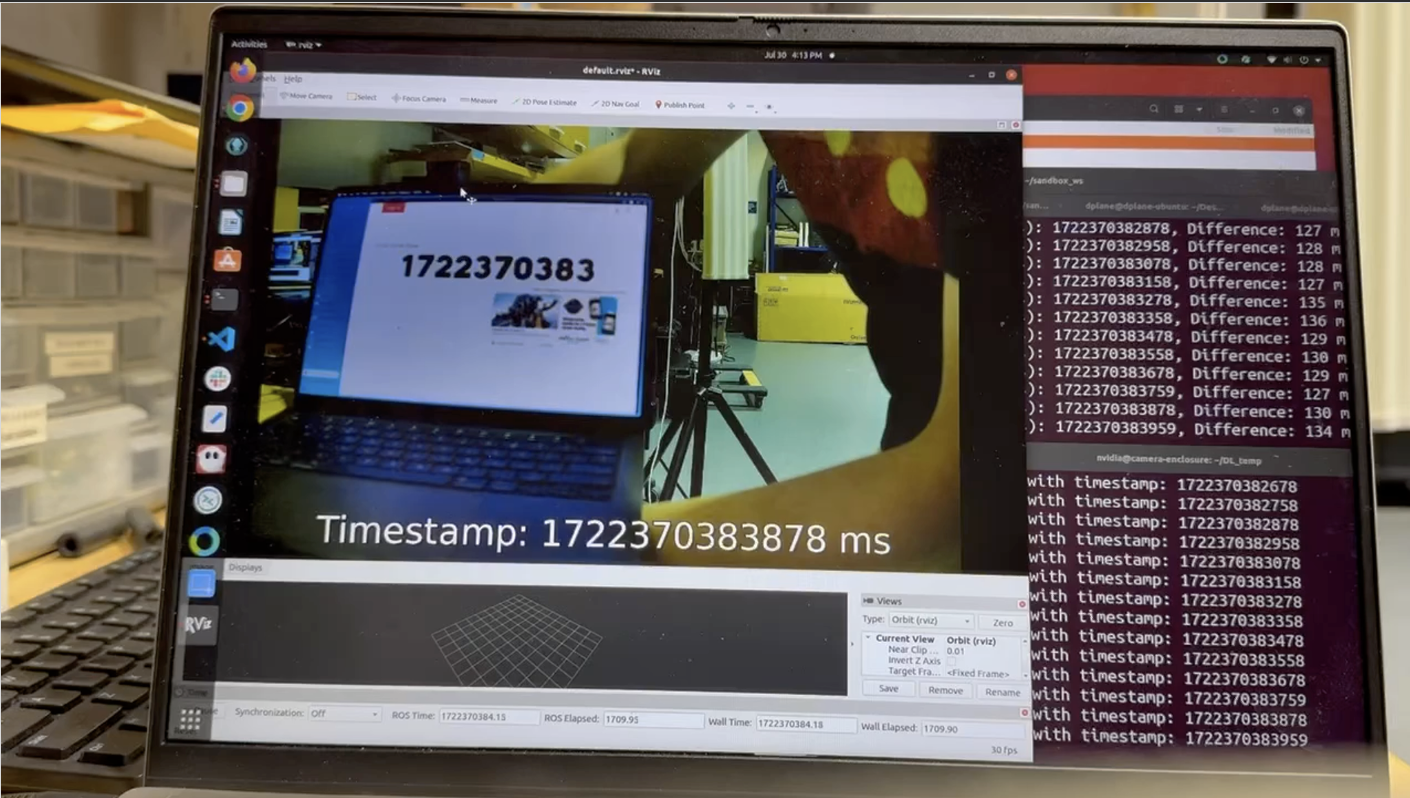
\includegraphics[width=0.8\linewidth]{Images/time_sync1.png}
    \caption{Testing the timestamp embedding within the RTSP stream for dropped frames and real-world temporal accuracy.}
    \label{fig:time_sync1}
\end{figure}
% Data was recorded by outputting the timestamps being sent and received by video camera, as well as by exporting this data to a log file on each machine. 

During the test, system-wide clock synchronization was measured using Chrony, which reported an average offset of $197;\text{ms};\pm;33;\text{ms}$ between the NVIDIA Jetson and Atlas machines.
The results of this test showed a total delay in video frame reception of 127 milliseconds, and logs between computers showed zero dropped frames with a 100\% match between timestamps.
\textcolor{blue}{This test was performed on Helios - Not Atlas, and did not have a true "master clock", if I recall. Find more recent test data. I would bet that running with updated chrony and ptp4l settings reduces this number significantly.}

Despite this result in frame delivery and timestamp assignment during testing, analysis of the recorded ROS bagfile data revealed a measurable drift between the original frame timestamps on the Jetson and those recorded by the Atlas system. 
% This discrepancy is believed to stem from thermal issues within the camera enclosure that were encountered during data collection.
% Therefore, some postprocessing of the data was required to ensure its validity.
This discrepancy is believed to result from thermal effects within the sealed camera enclosure during extended operation. 
Although no direct temperature measurements were recorded during this test, subsequent observations suggest that overheating may influence the Jetson's internal clock stability. 
This hypothesis remains unverified and will be revisited in Section~\ref{chap:recommendations}.

To resolve this, structural similarity (SSIM) scoring was employed to match each frame recorded by ROS on the Atlas to its corresponding source frame from the original video files on the Jetson. 
Although SSIM is conventionally used to assess visual degradation from compression, in this context, it served as a frame-matching metric: matched frames produced SSIM scores near 1.0, while mismatches scored closer to 0.0. The SSIM metric used is defined as:
\begin{equation}
    \text{SSIM}(x, y) = \frac{(2\mu_x\mu_y + C_1)(2\sigma_{xy} + C_2)}{(\mu_x^2 + \mu_y^2 + C_1)(\sigma_x^2 + \sigma_y^2 + C_2)}
\end{equation}

In this expression, $\mu_x$ and $\mu_y$ represent the mean pixel intensities of images $x$ and $y$, $\sigma_x^2$ and $\sigma_y^2$ are their variances, $\sigma_{xy}$ is the covariance between the images, and $C_1$ and $C_2$ are small constants that stabilize the division when the denominator is near zero.

To initialize alignment for each bag file, the first five ROS image messages within each bag were manually paired to the corresponding frames in the source video.
This established the offset the system was experiencing at the time the data was being recorded, which was then used to programmatically pair the remaining image messages in the bag with their video frame counterparts.
SSIM-based alignment was then automated on a subset of frames sampled at one-second intervals across each bagfile. 
Once alignment was confirmed through SSIM scores, the timestamps and frame indices for the intermediate frames were interpolated from the verified matches. 
Accordingly, the total number of frames analyzed by SSIM is approximately equal to the total number of seconds of recorded data.

To streamline this process across all 112 recorded bag files, a database was created to store file names, paths, and relevant metadata, allowing image and video data to be easily cross-referenced between the video and CSV files, and more than 100,000 ROS image messages. 
The same database also served as the repository for SSIM scores, interpolated matched frame numbers, and both the original and corrected timestamps for each image message. 
This dual-purpose design enabled automation of the SSIM alignment process while simultaneously providing a complete record of the aligned frame data for offline analysis and validation.


\end{document}